\documentclass[12pt,a4paper]{article}
\usepackage[utf8]{inputenc}
\usepackage[T1]{fontenc}
\usepackage{amsmath}
\usepackage{amsfonts}
\usepackage{amssymb}
\usepackage{graphicx}
\usepackage{hyperref}
\usepackage[polish]{babel}
\usepackage{algorithm}
\usepackage{algpseudocode}
\usepackage{booktabs}
\usepackage{float}

% Fix for Polish algorithm name
\makeatletter
\def\ALG@name{Algorytm}
\makeatother

% Allow algorithms to float but keep them in the same section
\floatplacement{algorithm}{tbp}

\title{Sprawozdanie z implementacji heurystyk konstrukcyjnych dla zmodyfikowanego problemu komiwojażera}
\author{Filip Rosiak 151799  \and Eryk Stec 152948}
\date{\today}

\begin{document}

\maketitle

\begin{abstract}
W niniejszym sprawozdaniu przedstawiono implementację i analizę heurystyk konstrukcyjnych dla zmodyfikowanego problemu komiwojażera. Problem polega na ułożeniu dwóch rozłącznych zamkniętych ścieżek, każda zawierająca około 50\% wierzchołków, minimalizując łączną długość obu ścieżek. Zaimplementowano i porównano cztery algorytmy: metodę najbliższego sąsiada, metodę rozbudowy cyklu, algorytm z 2-żalem oraz algorytm z ważonym 2-żalem. Eksperymenty przeprowadzono na instancjach kroa200 i krob200 z biblioteki TSPLib.
\end{abstract}

\section{Opis problemu}
Rozważany problem jest modyfikacją klasycznego problemu komiwojażera. Dany jest zbiór wierzchołków i symetryczna macierz odległości pomiędzy dowolną parą wierzchołków. Zadanie polega na ułożeniu dwóch rozłącznych zamkniętych ścieżek (cykli), każda zawierająca 50\% wierzchołków (jeżeli liczba wierzchołków w instancji nie jest parzysta, to pierwsza ścieżka zawiera jeden wierzchołek więcej), minimalizując łączną długość obu ścieżek.

Do testów wykorzystano instancje \texttt{kroa200} i \texttt{krob200} z biblioteki TSPLib. Są to dwuwymiarowe instancje euklidesowe, gdzie dla każdego wierzchołka podane są dwie współrzędne, a odległość pomiędzy wierzchołkami jest odległością euklidesową zaokrąglaną do liczby całkowitej.

\section{Zaimplementowane algorytmy}
W ramach zadania zaimplementowano następujące heurystyki konstrukcyjne:

\subsection{Algorytm najbliższego sąsiada}
Algorytm jest inspirowany metodą najbliższego sąsiada dla klasycznego problemu komiwojażera, dostosowany do rozważanego problemu z dwoma cyklami. Pseudokod algorytmu przedstawiono w Algorytmie~\ref{alg:nearest_neighbor}.

\begin{algorithm}
\caption{Algorytm najbliższego sąsiada dla zmodyfikowanego problemu komiwojażera}
\label{alg:nearest_neighbor}
\begin{algorithmic}[1]
\State \textbf{Znajdź punkty startowe:}
\State Znajdź parę wierzchołków $(s_1, s_2)$ z maksymalną odległością między nimi
\State Te wierzchołki będą punktami startowymi dla cykli $C_1$ i $C_2$

\State \textbf{Inicjalizuj cykle:}
\State $C_1 = [s_1]$
\State $C_2 = [s_2]$
\State Dostępne wierzchołki $A = \{0, 1, ..., n-1\} \setminus \{s_1, s_2\}$

\State \textbf{Naprzemiennie rozbudowuj cykle:}
\State $bieżący\_cykl = 1$ \Comment{Zaczynamy od cyklu 1}
\While{$A$ nie jest puste}
    \If{$bieżący\_cykl = 1$}
        \State Znajdź wierzchołek $v \in A$ najbliższy ostatniemu wierzchołkowi w $C_1$
        \State Dodaj $v$ do $C_1$
        \State Usuń $v$ z $A$
        \State $bieżący\_cykl = 2$
    \Else
        \State Znajdź wierzchołek $v \in A$ najbliższy ostatniemu wierzchołkowi w $C_2$
        \State Dodaj $v$ do $C_2$
        \State Usuń $v$ z $A$
        \State $bieżący\_cykl = 1$
    \EndIf
\EndWhile

\State \Return $(C_1, C_2)$
\end{algorithmic}
\end{algorithm}

\subsection{Algorytm rozbudowy cyklu}
Algorytm jest inspirowany metodą rozbudowy cyklu (greedy cycle) dla klasycznego problemu komiwojażera, dostosowany do rozważanego problemu z dwoma cyklami. Pseudokod algorytmu przedstawiono w Algorytmie~\ref{alg:greedy_cycle}.

\begin{algorithm}
\caption{Algorytm rozbudowy cyklu dla zmodyfikowanego problemu komiwojażera}
\label{alg:greedy_cycle}
\begin{algorithmic}[1]
\State \textbf{Znajdź punkty startowe:}
\State Znajdź parę wierzchołków $(s_1, s_2)$ z maksymalną odległością między nimi
\State Te wierzchołki będą punktami startowymi dla cykli $C_1$ i $C_2$

\State \textbf{Inicjalizuj cykle:}
\State $C_1 = [s_1]$
\State $C_2 = [s_2]$
\State Dostępne wierzchołki $A = \{0, 1, ..., n-1\} \setminus \{s_1, s_2\}$

\State \textbf{Dodaj początkowe wierzchołki do cykli:}
\If{$A$ nie jest puste}
    \State Znajdź wierzchołek $v_1 \in A$ najbliższy do $s_1$
    \State Dodaj $v_1$ do $C_1$ i usuń z $A$
    \If{$A$ nie jest puste}
        \State Znajdź wierzchołek $v_2 \in A$ najbliższy do $s_2$
        \State Dodaj $v_2$ do $C_2$ i usuń z $A$
    \EndIf
\EndIf

\State \textbf{Naprzemiennie rozbudowuj cykle:}
\State $bieżący\_cykl = 1$ \Comment{Zaczynamy od cyklu 1}
\While{$A$ nie jest puste}
    \If{$bieżący\_cykl = 1$}
        \For{każdy wierzchołek $v \in A$}
            \For{każdą pozycję $p$ w $C_1$}
                \State Oblicz koszt wstawienia $v$ na pozycję $p$ w $C_1$
            \EndFor
            \State Znajdź pozycję $p_v$ z minimalnym kosztem wstawienia dla $v$
        \EndFor
        \State Wybierz wierzchołek $v^*$ i pozycję $p^*$ z minimalnym kosztem wstawienia
        \State Wstaw $v^*$ na pozycji $p^*$ w $C_1$
        \State Usuń $v^*$ z $A$
        \State $bieżący\_cykl = 2$
    \Else
        \For{każdy wierzchołek $v \in A$}
            \For{każdą pozycję $p$ w $C_2$}
                \State Oblicz koszt wstawienia $v$ na pozycję $p$ w $C_2$
            \EndFor
            \State Znajdź pozycję $p_v$ z minimalnym kosztem wstawienia dla $v$
        \EndFor
        \State Wybierz wierzchołek $v^*$ i pozycję $p^*$ z minimalnym kosztem wstawienia
        \State Wstaw $v^*$ na pozycji $p^*$ w $C_2$
        \State Usuń $v^*$ z $A$
        \State $bieżący\_cykl = 1$
    \EndIf
\EndWhile

\State \Return $(C_1, C_2)$
\end{algorithmic}
\end{algorithm}

\subsection{Algorytm z 2-żalem}
Algorytm wykorzystuje koncepcję 2-żalu (2-regret) na bazie algorytmu rozbudowy cyklu. Pseudokod algorytmu przedstawiono w Algorytmie~\ref{alg:regret_cycle}.

\begin{algorithm}
\caption{Algorytm z 2-żalem dla zmodyfikowanego problemu komiwojażera}
\label{alg:regret_cycle}
\begin{algorithmic}[1]
\State \textbf{Znajdź punkty startowe:}
\State Znajdź parę wierzchołków $(s_1, s_2)$ z maksymalną odległością między nimi
\State Te wierzchołki będą punktami startowymi dla cykli $C_1$ i $C_2$

\State \textbf{Inicjalizuj cykle:}
\State $C_1 = [s_1]$
\State $C_2 = [s_2]$
\State Dostępne wierzchołki $A = \{0, 1, ..., n-1\} \setminus \{s_1, s_2\}$

\State \textbf{Dodaj początkowe wierzchołki do cykli:}
\If{$A$ nie jest puste}
    \State Znajdź wierzchołek $v_1 \in A$ najbliższy do $s_1$
    \State Dodaj $v_1$ do $C_1$ i usuń z $A$
    \If{$A$ nie jest puste}
        \State Znajdź wierzchołek $v_2 \in A$ najbliższy do $s_2$
        \State Dodaj $v_2$ do $C_2$ i usuń z $A$
    \EndIf
\EndIf

\State \textbf{Naprzemiennie rozbudowuj cykle:}
\State $bieżący\_cykl = 1$ \Comment{Zaczynamy od cyklu 1}
\While{$A$ nie jest puste}
    \If{$bieżący\_cykl = 1$}
        \For{każdy wierzchołek $v \in A$}
            \For{każdą pozycję $p$ w $C_1$}
                \State Oblicz koszt wstawienia $v$ na pozycję $p$ w $C_1$
            \EndFor
            \State Posortuj koszty rosnąco
            \State Oblicz 2-żal jako różnicę między drugim najlepszym a najlepszym kosztem
            \State Zapamiętaj najlepszą pozycję wstawienia dla $v$
        \EndFor
        \State Wybierz wierzchołek $v^*$ z największą wartością 2-żalu
        \State Wstaw $v^*$ na jego najlepszej pozycji w $C_1$
        \State Usuń $v^*$ z $A$
        \State $bieżący\_cykl = 2$
    \Else
        \For{każdy wierzchołek $v \in A$}
            \For{każdą pozycję $p$ w $C_2$}
                \State Oblicz koszt wstawienia $v$ na pozycję $p$ w $C_2$
            \EndFor
            \State Posortuj koszty rosnąco
            \State Oblicz 2-żal jako różnicę między drugim najlepszym a najlepszym kosztem
            \State Zapamiętaj najlepszą pozycję wstawienia dla $v$
        \EndFor
        \State Wybierz wierzchołek $v^*$ z największą wartością 2-żalu
        \State Wstaw $v^*$ na jego najlepszej pozycji w $C_2$
        \State Usuń $v^*$ z $A$
        \State $bieżący\_cykl = 1$
    \EndIf
\EndWhile

\State \Return $(C_1, C_2)$
\end{algorithmic}
\end{algorithm}

\subsection{Algorytm z ważonym 2-żalem}
Algorytm łączy koncepcję 2-żalu z regułą zachłanną, stosując wagi dla obu składników. Pseudokod algorytmu przedstawiono w Algorytmie~\ref{alg:weighted_regret}.

\begin{algorithm}
\caption{Algorytm z ważonym 2-żalem dla zmodyfikowanego problemu komiwojażera}
\label{alg:weighted_regret}
\begin{algorithmic}[1]
\State \textbf{Znajdź punkty startowe:}
\State Znajdź parę wierzchołków $(s_1, s_2)$ z maksymalną odległością między nimi
\State Te wierzchołki będą punktami startowymi dla cykli $C_1$ i $C_2$

\State \textbf{Inicjalizuj cykle:}
\State $C_1 = [s_1]$
\State $C_2 = [s_2]$
\State Dostępne wierzchołki $A = \{0, 1, ..., n-1\} \setminus \{s_1, s_2\}$

\State \textbf{Ustal wagi:} $w_r = 1.0$ (waga dla żalu), $w_g = -1.0$ (waga dla kosztu zachłannego)

\State \textbf{Dodaj początkowe wierzchołki do cykli:}
\If{$A$ nie jest puste}
    \State Znajdź wierzchołek $v_1 \in A$ najbliższy do $s_1$
    \State Dodaj $v_1$ do $C_1$ i usuń z $A$
    \If{$A$ nie jest puste}
        \State Znajdź wierzchołek $v_2 \in A$ najbliższy do $s_2$
        \State Dodaj $v_2$ do $C_2$ i usuń z $A$
    \EndIf
\EndIf

\State \textbf{Naprzemiennie rozbudowuj cykle:}
\State $bieżący\_cykl = 1$ \Comment{Zaczynamy od cyklu 1}
\While{$A$ nie jest puste}
    \If{$bieżący\_cykl = 1$}
        \For{każdy wierzchołek $v \in A$}
            \For{każdą pozycję $p$ w $C_1$}
                \State Oblicz koszt wstawienia $v$ na pozycję $p$ w $C_1$
            \EndFor
            \State Posortuj koszty rosnąco
            \State Oblicz najlepszy koszt wstawienia $c_1(v)$
            \State Oblicz drugi najlepszy koszt wstawienia $c_2(v)$
            \State Oblicz żal: $regret(v) = c_2(v) - c_1(v)$
            \State Oblicz ważoną ocenę: $score(v) = w_r \cdot regret(v) + w_g \cdot c_1(v)$
            \State Zapamiętaj najlepszą pozycję wstawienia dla $v$
        \EndFor
        \State Wybierz wierzchołek $v^*$ z najwyższą wartością ważonej oceny
        \State Wstaw $v^*$ na jego najlepszej pozycji w $C_1$
        \State Usuń $v^*$ z $A$
        \State $bieżący\_cykl = 2$
    \Else
        \For{każdy wierzchołek $v \in A$}
            \For{każdą pozycję $p$ w $C_2$}
                \State Oblicz koszt wstawienia $v$ na pozycję $p$ w $C_2$
            \EndFor
            \State Posortuj koszty rosnąco
            \State Oblicz najlepszy koszt wstawienia $c_1(v)$
            \State Oblicz drugi najlepszy koszt wstawienia $c_2(v)$
            \State Oblicz żal: $regret(v) = c_2(v) - c_1(v)$
            \State Oblicz ważoną ocenę: $score(v) = w_r \cdot regret(v) + w_g \cdot c_1(v)$
            \State Zapamiętaj najlepszą pozycję wstawienia dla $v$
        \EndFor
        \State Wybierz wierzchołek $v^*$ z najwyższą wartością ważonej oceny
        \State Wstaw $v^*$ na jego najlepszej pozycji w $C_2$
        \State Usuń $v^*$ z $A$
        \State $bieżący\_cykl = 1$
    \EndIf
\EndWhile

\State \Return $(C_1, C_2)$
\end{algorithmic}
\end{algorithm}

\section{Wyniki eksperymentów}
Każdy algorytm został uruchomiony 100 razy na instancjach kroa200 i krob200. Poniżej przedstawiono wyniki eksperymentów.

\begin{table}[H]
\centering
\caption{Wyniki eksperymentów dla instancji kroa200 i krob200}
\begin{tabular}{lcc}
\toprule
\textbf{Algorytm} & \textbf{kroa200} & \textbf{krob200} \\
\midrule
Najbliższy sąsiad & 44445 (44445 - 44445) & 45875 (45875 - 45875) \\
Rozbudowa cyklu & 38481 (38481 - 38481) & 39838 (39838 - 39838) \\
2-żal & 44734 (44734 - 44734) & 42612 (42612 - 42612) \\
Ważony 2-żal & 34826 (34826 - 34826) & 37496 (37496 - 37496) \\
\bottomrule
\end{tabular}
\end{table}

Warto zauważyć, że wartości średnie, maksymalne i minimalne dla każdej pary instancji i algorytmu są jednakowe. Wynika to z faktu, że wszystkie zaimplementowane algorytmy są deterministyczne, co oznacza, że dla tych samych danych wejściowych zawsze generują takie same rozwiązania.

\begin{table}[H]
\centering
\caption{Czasy wykonania algorytmów [ms]}
\begin{tabular}{lcc}
\toprule
\textbf{Algorytm} & \textbf{kroa200} & \textbf{krob200} \\
\midrule
Najbliższy sąsiad & 0.00 & 0.00 \\
Rozbudowa cyklu & 2.02 & 2.00 \\
2-żal & 8.65 & 9.06 \\
Ważony 2-żal & 8.17 & 8.44 \\
\bottomrule
\end{tabular}
\end{table}

\section{Wizualizacje}
Poniżej przedstawiono wizualizacje najlepszych rozwiązań dla każdej kombinacji algorytm/instancja.

\subsection{Instancja kroa200}

\begin{figure}[H]
\centering
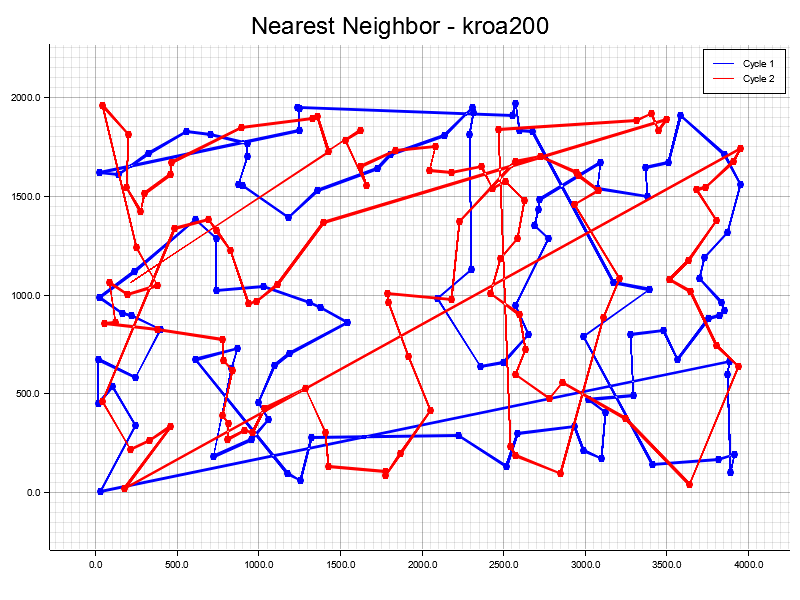
\includegraphics[width=0.8\textwidth]{figures/kroa200_Nearest_Neighbor.png}
\caption{Wizualizacja rozwiązania dla algorytmu najbliższego sąsiada na instancji kroa200}
\end{figure}

\begin{figure}[H]
\centering
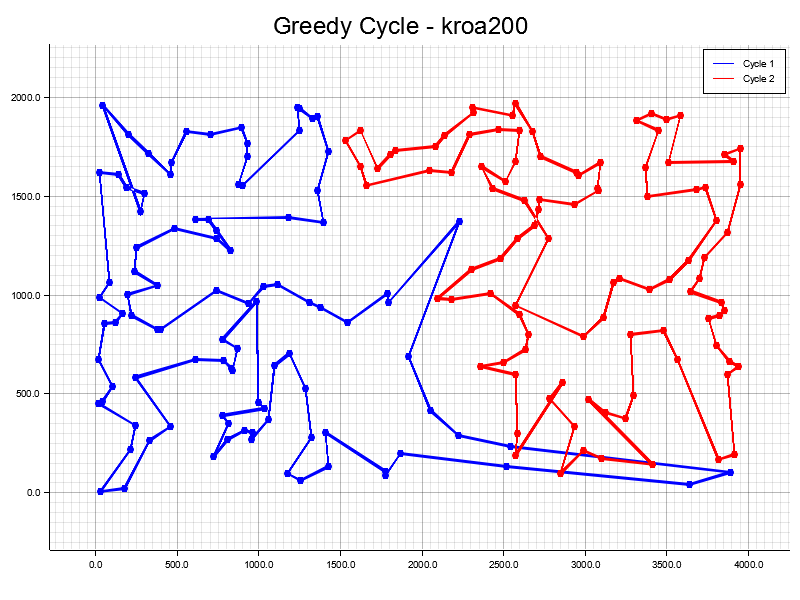
\includegraphics[width=0.8\textwidth]{figures/kroa200_Greedy_Cycle.png}
\caption{Wizualizacja rozwiązania dla algorytmu rozbudowy cyklu na instancji kroa200}
\end{figure}

\begin{figure}[H]
\centering
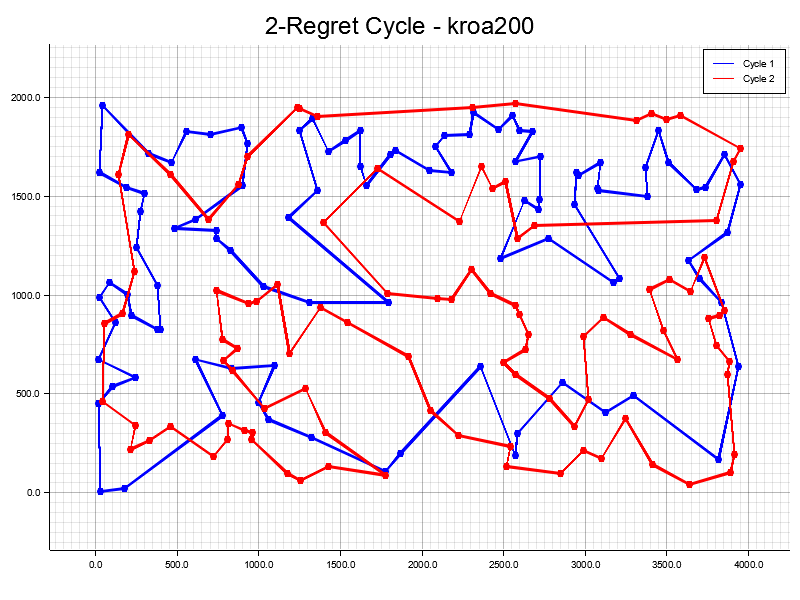
\includegraphics[width=0.8\textwidth]{figures/kroa200_2-Regret_Cycle.png}
\caption{Wizualizacja rozwiązania dla algorytmu z 2-żalem na instancji kroa200}
\end{figure}

\begin{figure}[H]
\centering
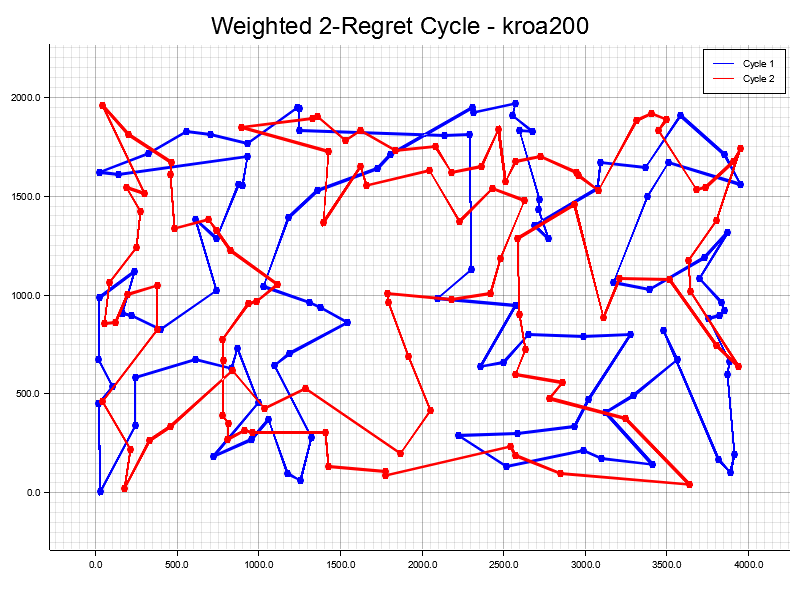
\includegraphics[width=0.8\textwidth]{figures/kroa200_Weighted_2-Regret_Cycle.png}
\caption{Wizualizacja rozwiązania dla algorytmu z ważonym 2-żalem na instancji kroa200}
\end{figure}

\subsection{Instancja krob200}

\begin{figure}[H]
\centering
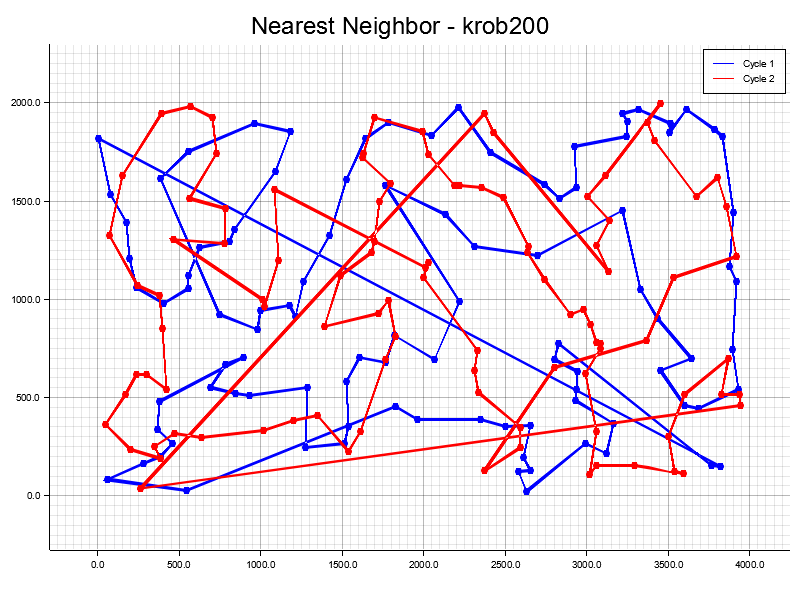
\includegraphics[width=0.8\textwidth]{figures/krob200_Nearest_Neighbor.png}
\caption{Wizualizacja rozwiązania dla algorytmu najbliższego sąsiada na instancji krob200}
\end{figure}

\begin{figure}[H]
\centering
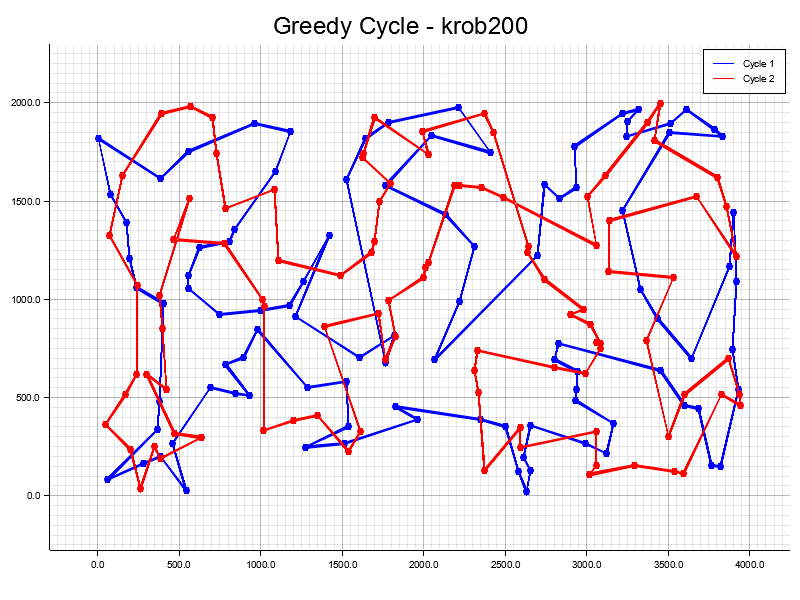
\includegraphics[width=0.8\textwidth]{figures/krob200_Greedy_Cycle.png}
\caption{Wizualizacja rozwiązania dla algorytmu rozbudowy cyklu na instancji krob200}
\end{figure}

\begin{figure}[H]
\centering
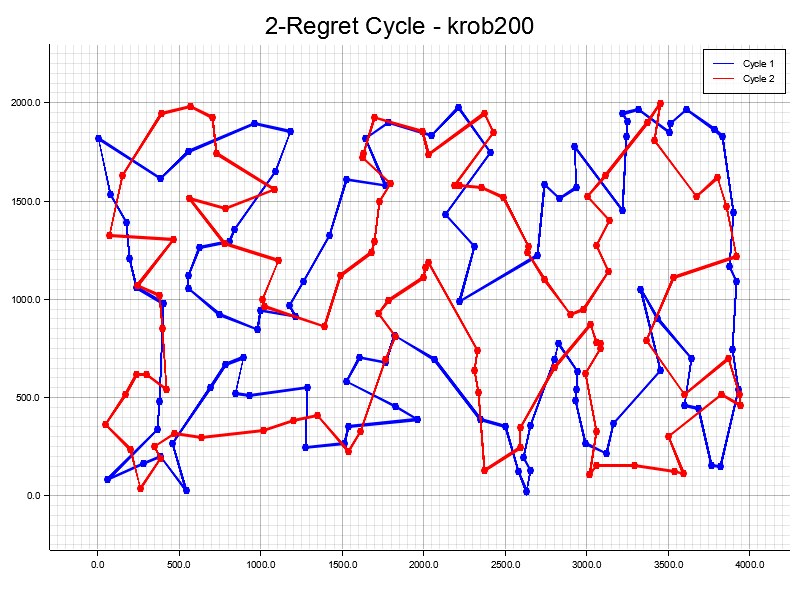
\includegraphics[width=0.8\textwidth]{figures/krob200_2-Regret_Cycle.png}
\caption{Wizualizacja rozwiązania dla algorytmu z 2-żalem na instancji krob200}
\end{figure}

\begin{figure}[H]
\centering
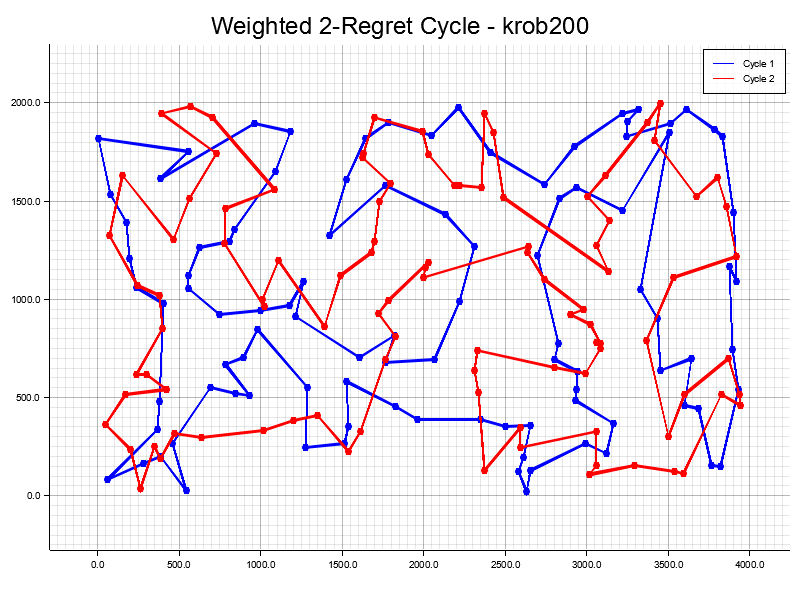
\includegraphics[width=0.8\textwidth]{figures/krob200_Weighted_2-Regret_Cycle.png}
\caption{Wizualizacja rozwiązania dla algorytmu z ważonym 2-żalem na instancji krob200}
\end{figure}

\section{Wnioski}
Na podstawie przeprowadzonych eksperymentów można wyciągnąć następujące wnioski:

\begin{enumerate}
    \item Algorytm z ważonym 2-żalem (Algorytm~\ref{alg:weighted_regret}) osiągnął najlepsze wyniki dla obu instancji, uzyskując najniższe koszty rozwiązań (34826 dla kroa200 i 37496 dla krob200).
    
    \item Algorytm najbliższego sąsiada (Algorytm~\ref{alg:nearest_neighbor}), mimo że jest najszybszy (czas wykonania bliski 0 ms), daje gorsze wyniki pod względem jakości rozwiązań (44445 dla kroa200 i 45875 dla krob200) niż algorytmy oparte na rozbudowie cyklu.
    
    \item Algorytm rozbudowy cyklu (Algorytm~\ref{alg:greedy_cycle}) oferuje dobry kompromis między jakością rozwiązania a czasem wykonania, osiągając wyniki lepsze niż algorytm najbliższego sąsiada przy niewielkim koszcie czasowym (około 2 ms).
    
    \item Algorytm z 2-żalem (Algorytm~\ref{alg:regret_cycle}), mimo podobnego czasu wykonania jak algorytm z ważonym 2-żalem, daje gorsze wyniki. Może to sugerować, że zastosowanie wag w algorytmie z ważonym 2-żalem pozwala na lepsze zrównoważenie między kosztem wstawienia a wartością żalu.
    
    \item Wszystkie algorytmy oparte na żalu (z 2-żalem i ważony 2-żal) wymagają znacznie więcej czasu obliczeniowego niż prostsze heurystyki, co jest spowodowane koniecznością obliczania i porównywania kosztów dla wszystkich możliwych pozycji wstawienia.
    
    \item Wizualizacje rozwiązań pokazują, że algorytmy oparte na żalu tworzą bardziej regularne i krótsze cykle, przy czym algorytm z ważonym 2-żalem generuje najlepsze rozwiązania pod względem całkowitej długości cykli.
\end{enumerate}

Podsumowując, wybór odpowiedniego algorytmu zależy od priorytetów: jeśli najważniejsza jest jakość rozwiązania, należy wybrać algorytm z ważonym 2-żalem; jeśli czas wykonania jest krytyczny, algorytm najbliższego sąsiada będzie najlepszym wyborem; natomiast algorytm rozbudowy cyklu stanowi rozsądny kompromis między jakością a czasem wykonania.

\section{Kod źródłowy}
Pełny kod źródłowy implementacji wszystkich algorytmów jest dostępny w repozytorium GitHub:
\url{https://github.com/Veanir/imo-1}

\end{document} 